\documentclass[a4paper]{tp_um}
\makeatletter
%--------------------------------------------------------------------------------

\usepackage[french]{babel}
\usepackage{amsmath}
\usepackage{amsbsy}
\usepackage{amsfonts}
\usepackage{amssymb}
\usepackage{amscd}
\usepackage{amsthm}
\usepackage{mathtools}
\usepackage{eurosym}
\usepackage{nicefrac}

\usepackage{latexsym}
\usepackage[a4paper,hmargin=20mm,vmargin=25mm]{geometry}
\usepackage{dsfont}
\usepackage[utf8]{inputenc}
\usepackage[T1]{fontenc}
\usepackage{lmodern}

\usepackage{multicol}
\usepackage[inline]{enumitem}
\setlist{nosep}
\setlist[itemize,1]{,label=$-$}


\newenvironment{modenumerate}
  {\enumerate\setupmodenumerate}
  {\endenumerate}

\newif\ifmoditem
\newcommand{\setupmodenumerate}{%
  \global\moditemfalse
  \let\origmakelabel\makelabel
  \def\moditem##1{\global\moditemtrue\def\mesymbol{##1}\item}%
  \def\makelabel##1{%
    \origmakelabel{##1\ifmoditem\rlap{\mesymbol}\fi\enspace}%
    \global\moditemfalse}%
}


\usepackage{sectsty}
%\sectionfont{}
\allsectionsfont{\color{astral}\normalfont\sffamily\bfseries\normalsize}

\usepackage{graphicx}
\usepackage{tikz}
\usetikzlibrary{babel}
\usepackage{tikz,tkz-tab}

\usepackage[babel=true, kerning=true]{microtype}


\usepackage{pgfplots}
\usepgfplotslibrary{fillbetween}
\pgfplotsset{compat=newest}
\usepgfplotslibrary{external} 
\tikzexternalize[prefix=./output_latex/]
%\DeclareSymbolFont{RalphSmithFonts}{U}{rsfs}{m}{n}
%\DeclareSymbolFontAlphabet{\mathscr}{RalphSmithFonts}
%\def\mathcal#1{{\mathscr #1}}



\providecommand{\abs}[1]{\left|#1\right|}
\providecommand{\norm}[1]{\left\Vert#1\right\Vert}
\providecommand{\U}{\mathcal{U}}
\providecommand{\R}{\mathbb{R}}
\providecommand{\Cc}{\mathcal{C}}
\providecommand{\reg}[1]{\mathcal{C}^{#1}}
\providecommand{\1}{\mathds{1}}
\providecommand{\N}{\mathbb{N}}
\providecommand{\Z}{\mathbb{Z}}
\providecommand{\p}{\partial}
\providecommand{\one}{\mathds{1}}
\providecommand{\E}{\mathbb{E}}\providecommand{\V}{\mathbb{V}}
\renewcommand{\P}{\mathbb{P}}


%Operateur
\providecommand{\abs}[1]{\left\lvert#1\right\rvert}
\providecommand{\sabs}[1]{\lvert#1\rvert}
\providecommand{\babs}[1]{\bigg\lvert#1\bigg\rvert}
\providecommand{\norm}[1]{\left\lVert#1\right\rVert}
\providecommand{\bnorm}[1]{\bigg\lVert#1\bigg\rVert}
\providecommand{\snorm}[1]{\lVert#1\rVert}
\providecommand{\prs}[1]{\left\langle #1\right\rangle}
\providecommand{\sprs}[1]{\langle #1\rangle}
\providecommand{\bprs}[1]{\bigg\langle #1\bigg\rangle}

\DeclareMathOperator{\deet}{Det}
\DeclareMathOperator{\hess}{Hess}
\DeclareMathOperator{\jac}{Jac}


\newcommand\rst[2]{{#1}_{\restriction_{#2}}}



% generate breakable white space allowing students to write notes.

\usepackage[framemethod=tikz]{mdframed}

\mdfdefinestyle{response}{
	leftmargin=.01\textwidth,
	rightmargin=.01\textwidth,
	linewidth=1pt
	hidealllines=false,
	leftline=true,
	rightline=true,topline=true,bottomline=true,
	skipabove=0pt,
	%innertopmargin=-5pt,
	%innerbottommargin=2pt,
	linecolor=black,
	innerrightmargin=0pt,
	}



\newcommand*{\DivideLengths}[2]{%
  \strip@pt\dimexpr\number\numexpr\number\dimexpr#1\relax*65536/\number\dimexpr#2\relax\relax sp\relax
}

\providecommand{\rep}[1]{$ $ \newline \begin{mdframed}[style=response]  
	
	\vspace*{\DivideLengths{#1}{3cm}cm}
	\pagebreak[1]	
	\vspace*{\DivideLengths{#1}{3cm}cm}
	\pagebreak[1]		
	\vspace*{\DivideLengths{#1}{3cm}cm}   \end{mdframed}}

\providecommand{\blanc}[1]{$ $ \newline 
	
	\vspace*{\DivideLengths{#1}{3cm}cm}
	\pagebreak[1]	
	\vspace*{\DivideLengths{#1}{3cm}cm}
	\pagebreak[3]		
	\vspace*{\DivideLengths{#1}{3cm}cm}}

\usepackage{ifthen}

\newcommand{\eno}[1]{%
	\ifthenelse{\equal{\version}{eno}}{#1}{}%
}
\newcommand{\cor}[1]{%
        \ifthenelse{\equal{\version}{cor}}{
\medskip 

{\small \color{gray} #1}

\medskip 
}{}
}

%------------------------------------------------------------------------------
%\DeclareUnicodeCharacter{00A0}{~}
\makeatother



\usepackage[inline]{asymptote}
\usepackage{pdfpages}

% \def\version{eno}
\def\version{cor}

\ue{HLMA410}
%-----------------------------------------------------------------------------

\title{\large \sffamily\bfseries Contrôle continu 1}

\begin{document}

\maketitle
\textit{Durée 1h10. Les documents, la calculatrice, les téléphones portables, tablettes, ordinateurs ne sont pas autorisés. La qualité de la rédaction sera prise en compte.} 

\bigskip
\bigskip

\exo{} Soit $N : \R^2 \to \R$, définie pour $u = (x, y)$ par $N (u) = \sup_{0\leq t \leq 1} |x + ty|$
\begin{enumerate}
    \item Montrer que $N$ est une norme.

        \cor{
            Dans cette question $u = (x, y)$ et $v = (x_0 , y_0 )$ sont deux éléments quelconques de $\R^2$.
            \begin{itemize}
                \item La borne supérieure $N (u)$ existe car elle représente le maximum (atteint au moins pour une valeur $t_0$) de l'application $t \mapsto |x + ty|$, définie et continue sur $[0, 1]$.
                \item On a évidemment l’inégalité $N (x, y) \geq 0$.  D'autre part $N (x, y) = 0 \Rightarrow \forall t \in [0, 1], x + ty = 0 \Rightarrow x = y = 0$ (choisir $t = 0$ et $t = 1$.)
                \item Pour tout réel $\lambda$:
                    \[
                        N (\lambda u) = \sup_{0\leq t \leq 1} |(\lambda x) + t(\lambda y)| = \sup_{0\leq t \leq 1} |\lambda | |x + ty| = |\lambda | \sup_{0\leq t \leq 1} |x + ty| = |\lambda | N (u)
                    \]
                \item Pour tout réel $t$ de $[0, 1]$, $|(x + x_0 ) + t(y + y_0 )| \leq |x + ty| + |x_0 + ty_0 | \leq N (u) + N (v)$.
                    On peut alors passer à la borne supérieure dans $|(x + x_0 ) + t(y + y_0 )|$ et écrire :
            $N (u + v) \leq N (u) + N (v)$\end{itemize}
            L'application $u \mapsto N (u)$ est donc une norme sur $\R^2$.
        }

        \eno{
            \vspace*{13cm} \vfill
        }

    \item Représenter la boule unité fermée de centre 0. Justifier.

        \bigskip

        \begin{minipage}{.4\textwidth}
            \begin{tikzpicture}\pgfplotsset{compat=1.8}
                \begin{axis}[height=8cm,width=8cm,enlargelimits=true, axis lines=center, axis on top, xlabel={$x$}, ylabel={$y$}, axis equal,
                    ymin=-2.2,ymax=2.2,xmin=-1.2,xmax=1.2,grid=both, minor tick num=2,]

                    \cor{
                        \addplot[samples=5, very thick,red, domain = -1:1, samples y =0] ({1},{-1+x});
                        \addplot[samples=5, very thick,red, domain = -1:1, samples y =0] ({-1},{1+x});
                        \addplot[samples=5, very thick,red, domain = -1:1, samples y =0] ({x},{1-x});
                        \addplot[samples=5, very thick,red, domain = -1:1, samples y =0] ({x},{-1-x});
                    }
                \end{axis}  
            \end{tikzpicture}
        \end{minipage}\hfill
        \begin{minipage}[]{.4\textwidth}
            \cor{
                Soit $u = (x, y)$ un élément quelconque de $\R^2$, et soit $\phi$ définie sur $[0, 1]$ par  $\phi(t) = |x + ty|$. L’application positive $\phi^2$ est convexe sur 
                [$0, 1]$ (sa dérivée seconde est positive ou nulle).
                L’application $\phi^2$ atteint donc son maximum en $t = 0$ ou en $t = 1$. Il en est de même de $\phi$. On a donc :

                \begin{align*}
                    N(u) \leq 1 &\Leftrightarrow \begin{cases}
                        \phi(0) \leq 1\\ \phi(1) \leq 1
                    \end{cases}\\
                    & \Leftrightarrow
                    \begin{cases}
                        |x| \leq 1 \\
                        |x+y| \leq 1
                    \end{cases} \\ &\Leftrightarrow
                    \begin{cases}
                        -1 \leq x \leq 1\\ -x-1 \leq y \leq -x +1
                    \end{cases}
                \end{align*}
            }
        \end{minipage}
\end{enumerate}

\eno{
    \newpage
}

\exo{(Courbe de Viviani)} Dans cet exercice, on se propose d'étudier la courbe:
\begin{center}
    \begin{minipage}{.4\textwidth}
        \begin{tikzpicture}\pgfplotsset{compat=1.8}
\tikzstyle{every node}=[font=\small]
            \begin{axis}[height=4cm,width=4cm,enlargelimits=true, %axis lines=middle,
                xlabel={\small $x$}, ylabel={\small $y$}, zlabel={\small $z$}, axis equal, ymin=-1,ymax=1.0,xmin=-1.0,xmax=1, zmin=-1.0, zmax=1,grid=both, minor tick num=1, view={40}{15}]
                \addplot3[samples=500, very thick,red, domain = -pi:pi, samples y =0] ({cos(deg(x))^2},{cos(deg(x))*sin(deg(x))},{sin(deg(x))});
            \end{axis}	
        \end{tikzpicture}
    \end{minipage}
    \begin{minipage}{.55\textwidth}
    Dont une paramamétrisation est  pour tout $t\in ]-\pi,\pi[$ \[\phi:t\mapsto
            \begin{pmatrix}
                x(t) & = &\cos^2 t \\
                y(t) & = &\sin t \cos t \\
                z(t) & = &\sin t
        \end{pmatrix}\]
    \end{minipage}
\end{center}

\begin{enumerate}
    \item On considère la projection sur le plan $yz$. Soit donc la courbe paramétrée  $\phi_{yz}:t \mapsto \begin{pmatrix} y(t) \\ z(t) \end{pmatrix}$. 
        \begin{enumerate}
            \item Déterminer les points de $\phi_{yz}$ admettant, dans le plan $yz$, une tangente horizontale ou une tangente verticale

                \cor{Avant de commencer, on remarque que $y$ et $z$ sont impaires et la courbe admet donc une symétrie centrale par rapport à l'origine $O$ et deux symétries axiales par rapport à chacun des axes $Oy$ et $Oz$. 

                    On a $\phi'_{yz}(t) = \begin{pmatrix} y'(t) = \cos^2 t - \sin^2(t) \\ z'(t) = \cos t\end{pmatrix}$. Les tangentes verticales sont en les points pour lesquels  $y'(t) = 0$ et $z'(t)\neq 0$ (\textit{i.e.} pour $t=\pm \pi/4, \pm 3\pi/4$) et les tangentes horizontales sont en les points pour lesquels $z'(t)=0$ et $y'(t)\neq 0$ (\textit{i.e.} pour $t=\pm \pi/2$).

                }

                \eno{
                    \vspace*{5cm}
                }

            \item Compléter le tableau de variations suivant pour $\phi_{yz}$:
                \begin{center}
                    \eno{
                        \hspace*{-6em} \begin{tabular}{|c|ccccccccccccccccc|}
                            \hline  $t$  & $-\pi$ & \hspace{.3cm}& $-3\pi/4$ & \hspace{.3cm} & $-\pi/2$& \hspace{.3cm} & $-\pi/4$& \hspace{.3cm}  &  0	& \hspace{.3cm} & $\pi/4$ & \hspace{.3cm}   & $\pi/2$ & \hspace{.3cm} & $3\pi/4$ & \hspace{.3cm} & $\pi$ \\[0.3cm]\hline\hline
                            \begin{minipage}{3.3em}{\small signe de $y'(t)$}\end{minipage} &&&&&&&&&&&&&&&&&	\\[0.4cm]\hline
                            \begin{minipage}{3.3em}{\small variation de $y(t)$}\end{minipage} &&&&&&&&&&&&&&&&&	\\[0.4cm]\hline
                            \begin{minipage}{3.3em}{\small signe de $z'(t)$}\end{minipage} &&&&&&&&&&&&&&&&&	\\[0.4cm]\hline
                            \begin{minipage}{3.3em}{\small variation de $z(t)$}\end{minipage} &&&&&&&&&&&&&&&&&	\\[0.4cm]\hline
                        \end{tabular}
                    }
                    \cor{
                        {\small \hspace*{-6em} \begin{tabular}{|c|ccccccccccccccccc|}
                                \hline  $t$  & $-\pi$ & \hspace{.3cm}& $-3\pi/4$ & \hspace{.3cm} & $-\pi/2$& \hspace{.3cm} & $-\pi/4$& \hspace{.3cm}  &  0	& \hspace{.3cm} & $\pi/4$ & \hspace{.3cm}   & $\pi/2$ & \hspace{.3cm} & $3\pi/4$ & \hspace{.3cm} & $\pi$ \\[0.3cm]\hline\hline
                                \begin{minipage}{3.3em}{\small signe de $y'(t)$}\end{minipage} &&$+$&0&$-$&&$-$&0&+&&+&0&$-$&&$-$&0&+&	\\[0.4cm]\hline
                                \begin{minipage}{3.3em}{\small variation de $y(t)$}\end{minipage} &0&$\nearrow$&$1/2$&$\searrow$&0&$\searrow$&$-1/2$&$\nearrow$&0&$\nearrow$&$1/2$&$\searrow$&0&$\searrow$&$-1/2$&$\nearrow$&0	\\[0.4cm]\hline
                                \begin{minipage}{3.3em}{\small signe de $z'(t)$}\end{minipage} &&$-$&&$-$&0&+&&+&&+&&+&0&$-$&&$-$&	\\[0.4cm]\hline
                                \begin{minipage}{3.3em}{\small variation de $z(t)$}\end{minipage} &0&$\searrow$&$-\sqrt2/2$&$\searrow$&$-1$&$\nearrow$&$-\sqrt2/2$&$\nearrow$&0&$\nearrow$&$\sqrt2/2$&$\nearrow$&1&$\searrow$&$\sqrt2/2$&$\searrow$&0	\\[0.4cm]\hline
                        \end{tabular}}
                    }
                \end{center}

                \eno{
                    \vfill
                }

            \item Tracer la courbe $\phi_{yz}$ ainsi que ses tangentes:
                \begin{center}
                    \begin{tikzpicture}\pgfplotsset{compat=1.8}
                        \begin{axis}[height=7.0cm,width=7.0cm, axis lines=center, axis on top, xlabel={$y$}, ylabel={$z$}, axis equal,
                            ymin=-1.1,ymax=1.1,xmin=-1.1,xmax=1.1,grid=both, minor tick num=2]

                            \cor{
                                \addplot[samples=500, very thick,red, domain = -pi:pi, samples y =0] ({cos(deg(x))*sin(deg(x))},{sin(deg(x))});
                                \addplot[samples=5,<->, very thick,black, domain = -.3:.3, samples y =0] ({.5},{x+sqrt(2)/2});
                                \addplot[samples=5,<->, very thick,black, domain = -.3:.3, samples y =0] ({-.5},{x+sqrt(2)/2});
                                \addplot[samples=5,<->, very thick,black, domain = -.3:.3, samples y =0] ({.5},{x-sqrt(2)/2});
                                \addplot[samples=5,<->, very thick,black, domain = -.3:.3, samples y =0] ({-.5},{x-sqrt(2)/2});
                                \addplot[samples=5,<->, very thick,black, domain = -.3:.3, samples y =0] ({x},{1});
                                \addplot[samples=5,<->, very thick,black, domain = -.3:.3, samples y =0] ({x},{-1});
                            }
                        \end{axis}	
                    \end{tikzpicture}
                \end{center}
        \end{enumerate}

    \item \label{q1} On se place maintenant dans le plan $xy$. Calculer $\norm{\begin{pmatrix}
                x(t) - 1/2\\ y(t)
        \end{pmatrix}}$. Quelle interprétation géométrique peut-on faire? 

        \cor{
            On a 
            \begin{align*}
                (x(t) - 1/2)^2 + y^2(t) & =  \cos^4(t) - \cos^2(t) + 1/4  + \sin^2(t)\cos^2(t) \\ &=  -\cos^2(t)\sin^2(t) + 1/4 + \cos^2(t)\sin^2(t) = 1/4
            \end{align*}
            La courbe  $\phi_{xy}$ appartient donc au cercle de centre $(x,y) = (1/2,0)$ et de rayon $1/2$.
        }



        \eno{
            \vspace*{5cm}
        }


    \item On se place dans le plan $xz$. On considère alors $\phi_{xz}(t) =\begin{pmatrix} x(t)\\z(t) \end{pmatrix}$.
        \begin{enumerate}
            \item Trouver les points critiques de $\phi_{xz}$.


                \cor{
                    On a $x'(t) = 2 \sin t \cos t$ qui s'annule en $t = \pm \pi/2, 0$. Comme $z'(t)$ s'annule aussi en $\pm\pi/2$, il y a 2 points critiques.
                }

                \eno{
                    \vspace*{5cm}
                }

            \item Compléter le tableau de variation suivant pour $\phi_{xz}$:
                \begin{center}
                    \cor{
                        \hspace*{-6em} \begin{tabular}{|c|ccccccccc|}
                            \hline  $t$  & $-\pi$ & \hspace{1.5cm} & $-\pi/2$& \hspace{1.5cm} &    0	&  \hspace{1.5cm}   & $\pi/2$ & \hspace{1.5cm} & $\pi$ \\[0.3cm]\hline\hline
                            \begin{minipage}{3.3em}{\small signe de $x'(t)$}\end{minipage} &0& $-$ &0& $+$ & 0& $-$ &0 & $+$ &0	\\[0.4cm]\hline
                            \begin{minipage}{3.3em}{\small variation de $x(t)$}\end{minipage} &1 & $\searrow$ & 0& $\nearrow$  &1&  $\searrow$ & 0& $\nearrow$ &1	\\[0.4cm]\hline
                            \begin{minipage}{3.3em}{\small signe de $z'(t)$}\end{minipage} && $-$ & 0 & $+$ & & +& 0 & $-$ &	\\[0.4cm]\hline
                            \begin{minipage}{3.3em}{\small variation de $z(t)$}\end{minipage} &0&$\searrow$& $-1$ & $\nearrow$ & 0 & $\nearrow$ & 1 & $\searrow$ &0	\\[0.4cm]\hline
                        \end{tabular}
                    }
                    \eno{
                        \hspace*{-6em} \begin{tabular}{|c|ccccccccc|}
                            \hline  $t$  & $-\pi$ & \hspace{1.5cm} & $-\pi/2$& \hspace{1.5cm} &    0	&  \hspace{1.5cm}   & $\pi/2$ & \hspace{1.5cm} & $\pi$ \\[0.3cm]\hline\hline
                            \begin{minipage}{3.3em}{\small signe de $x'(t)$}\end{minipage} &&&&&&&&&	\\[0.4cm]\hline
                            \begin{minipage}{3.3em}{\small variation de $x(t)$}\end{minipage} &&&&&&&&&	\\[0.4cm]\hline
                            \begin{minipage}{3.3em}{\small signe de $z'(t)$}\end{minipage} &&&&&&&&&	\\[0.4cm]\hline
                            \begin{minipage}{3.3em}{\small variation de $z(t)$}\end{minipage} &&&&&&&&&	\\[0.4cm]\hline
                        \end{tabular}
                    }
                \end{center}
            \item Étudier la nature des points critiques de $\phi_{xz}$. On admettra que $\phi_{xz}(\pi/2 +t) =  \begin{pmatrix} (1 - \cos(2t))/2 \\ \cos(t) \end{pmatrix}$.


                \cor{
                    On remarque que la courbe admet une symétrie axiale par rapport à l'axe $Ox$. On peut donc se contenter d'étudier le point critique correspondant à $t=\pi/2$. On écrit le développement de Taylor
                    \begin{align*}
                        \phi_{xz}(\pi/2 +h ) &= \begin{pmatrix}
                            ( (2h)^2 /2 - (2h)^4 /4! + o(h^4))/2 \\
                            1 - h^2/2 + h^4/4! + o(h^4)
                        \end{pmatrix} \\ &= 
    %\begin{pmatrix}
    %     & h^2 &- h^4/3  &+ o(h^4) \\
    %     1  & -h^2/2 & + h^4/24 & + o(h^4)
    % \end{pmatrix} = 
                        \begin{pmatrix}
                            0\\1
                        \end{pmatrix} + \begin{pmatrix}
                            1\\-1/2
                        \end{pmatrix}h^2 + \begin{pmatrix}
                            -1/3\\1/24
                        \end{pmatrix} h^4 + \begin{pmatrix}
                            1\\1
                        \end{pmatrix} o(h^4)
                    \end{align*}
                    Avec les notations du cours on a $p=2$, $q=4$, la tangente est alors la droite portée par $v = (1, -1/2)$ et on a $w = (-1/3, 1/24) $. C'est donc un point de rebroussement de deuxième espèce:
                    \begin{center}
                        \begin{tikzpicture}[scale=1]
                            \begin{scope}[rotate=0] 
                                \draw[->, thick, red] (0,0)--(1,-.5) node[above] {${v}$}; 
                                \draw[->, thick, red] (0,0)--(-1/3,1/24) node[above] {${w}$}; 
                                \draw [>->,>=latex,very thick, color=blue] (1,-1) .. controls (0.2,0) and (0.2,-.1) .. (0,0) .. controls (0.3,-0.15) and (0.25,0) .. (.4,-1);
                                \fill (0,0) circle (1pt);
                            \end{scope}
                        \end{tikzpicture}
                    \end{center}
                }


                \eno{
                    \vfill
                    \vspace*{6cm}
                }

            \item Tracer la courbe de $\phi_{xz}$ ainsi que les tangentes en les points critiques.                        
                \begin{center}
                    \begin{tikzpicture}\pgfplotsset{compat=1.8}
                        \begin{axis}[height=7cm,width=7cm, axis lines=center, axis on top, xlabel={$x$}, ylabel={$z$}, axis equal,
                            ymin=-1.1,ymax=1.1,xmin=-1.1,xmax=1.1,grid=both, minor tick num=2]
                            \cor{
                                \addplot[samples=500, very thick,red, domain = -pi:pi, samples y =0] ({cos(deg(x))*cos(deg(x))},{sin(deg(x))});
                                \addplot[samples=5,->, very thick,black, domain = 0:.3, samples y =0] ({1*x},{ 1-x/2});
                                \addplot[samples=5,->, very thick,black, domain = 0:.3, samples y =0] ({1*x},{ -1+x/2});
                            }
                        \end{axis}  
                    \end{tikzpicture}
                \end{center}
        \end{enumerate}

    \item Retour dans $\R^3$. 

        \begin{enumerate}
            \item \label{q2} Calculer $\snorm{\phi(t)}$. Quelle interprétation géométrique peut on faire?


                \cor{
                    On a 
                    \begin{align*}
                        x^2(t) + y^2(t) + z^2(t)  &=  \cos^4 t + \sin^2 t \cos^2 t + \sin^2 t \\
                        & = \cos^2 t(1 - \sin^2 t)  + \sin^2 t \cos^2 t + \sin^2 t \\
                        & =  1
                    \end{align*}
                    Les points $\phi(t)$ sont donc portés par la sphère unitée centrée en l'origine.
                }

                \eno{
                    \vspace*{6cm}
                }
            \item Les questions \ref{q1} et \ref{q2} nous apprennent que la courbe  $\phi$ est à l'intersection de 2 objets géométriques simples. Lesquels? justifier.

                \cor{
                    La courbe $\phi$ est à l'intersection de la sphère unité centrée en l'origine et du cylindre de rayon $1/2$ et de droite de révolution vertical passant par le point $(1/2,0,0)$.
                    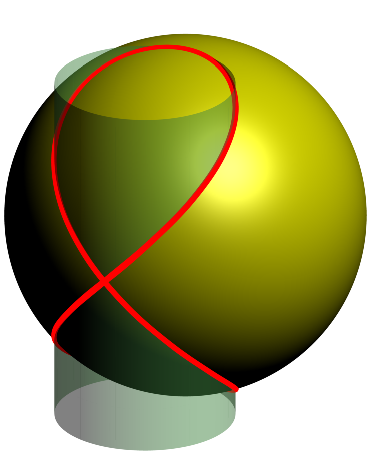
\includepdf[width=.6\textwidth]{sphere.pdf}
                    %\begin{asy}
                        %import three;

                        %size(200);
                        %currentprojection=orthographic(4,2,2);

                        %draw(unitsphere,yellow,render(compression=Zero,merge=true));

                        %import solids;

                        %real r=.5;
                        %real h=2;

                        %revolution R=cylinder(-h/2*Z,r,h);
                        %draw(shift(.5,0,0) * surface(R),lightgreen+opacity(0.5),render(compression=Zero));

                        %import graph3;
                        %triple f(real t) { return (cos(t)*cos(t), cos(t)*sin(t), sin(t)); }

                        %path3 Viviani = graph(f, -pi, pi, operator ..);
                        %draw(Viviani, red+linewidth(3));
                    %\end{asy}
                }


                \eno{
                    \vfill
                }
        \end{enumerate}
\end{enumerate}


\end{document}
